\documentclass[CJK]{beamer}
\usepackage{beamerthemesplit}
\usetheme{Hannover}  % ok2 
\usecolortheme{dolphin}
\usepackage[utf8]{inputenc}
\setbeamertemplate{footline}{\hfill\insertframenumber/\inserttotalframenumber}
\usepackage[BoldFont,SlantFont,CJKnumber]{xeCJK}
\usepackage{amsthm}
\usepackage{multirow}
\usepackage{amssymb}
\usepackage{fontspec}
\usepackage{float}
\usepackage{color,xcolor}
\usepackage{listings}
\usepackage{tikz}
\setsansfont{SimSun}
\title{编译体系联合实习结题报告}
\author{张番栋 00848180\\ 刘澜涛 00848200 \\王 沛 00848205}
\date{2010年12月29日}
\AtBeginSection[]
{
  \begin{frame}<beamer>{目录}
    \tableofcontents[currentsection]
  \end{frame}
}

\begin{document}

\frame{\titlepage}
\frame{\frametitle{目录}\tableofcontents}

\section{实习题目}
\subsection*{题目信息}
\frame{
  \frametitle{题目信息}
  \begin{tabular}{r|l}
    \hline
    题目 & 编译与体系结构联合实习 \\
    \hline
    \multirow{2}{*}{内容一} & 编写C语言子集的编译器 \\
    & 目标机为UniCore2处理器 \\
    \hline
    \multirow{2}{*}{内容二} & 编写支持UniCore2指令系统\\
    & 子集的模拟器 \\
    \hline
    内容三 & 编译器和模拟器能够协同工作 \\
    \hline
  \end{tabular}
}

\frame{
  \frametitle{实习目的}
  \begin{itemize}
  \item 深入理解编译器构造及实现
  \item 增加对计算机体系结构的认识
  \item 体会编译与体系结构之间的联系
  \end{itemize}
}
\section{小组介绍}
\subsection*{小组成员}
\frame{
  \frametitle{小组成员}
  \begin{itemize}
  \item 张番栋 00848180
  \item 刘澜涛 00848200
  \item 王 沛 00848205
  \end{itemize}
}
\subsection*{成员分工}
\frame{
  \frametitle{张番栋主要负责内容}
  \begin{itemize}
  \item 符号表
  \item 活跃变量分析
  \item 参与了目标代码生成
  \item 指令强度优化
  \end{itemize}
}
\frame{
  \frametitle{刘澜涛主要负责内容}
  \begin{itemize}
  \item 编译部分
    \begin{itemize}
    \item 参与建立符号表
    \item 中间代码生成表达式以上部分
    \item 基本块划分及流图化简
    \item 指针分析
    \item 参与目标代码生成
    \item 窥孔优化
    \end{itemize}
  \item 模拟器部分
    \begin{itemize}
    \item cache
    \end{itemize}
  \end{itemize}
}
\frame{
  \frametitle{王沛主要负责内容}
  \begin{itemize}
  \item 编译器部分
    \begin{itemize}
    \item 词法分析
    \item 语法树构建
    \item 语义检查
    \item 三元式生成
    \item 寄存器分配
    \end{itemize}
  \item 模拟器部分
    \begin{itemize}
    \item 编码与测试
    \end{itemize}
  \end{itemize}
}
\section{模拟器}
\frame{
  \frametitle{模拟器模块划分}
  \begin{enumerate}
  \item 存储管理模块
  \item 装载模块
  \item 流水线
  \end{enumerate}
}
\subsection*{存储管理}
\frame{
  \frametitle{页式内存管理}
  寻址方式
  \begin{figure}[H]
    \centering
    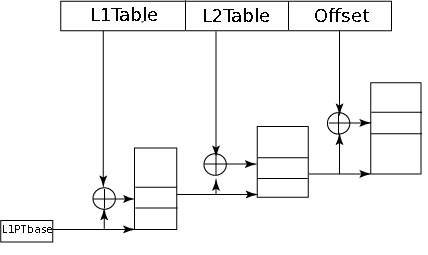
\includegraphics[width=0.4\textwidth]{pt.png}
  \end{figure}
  逻辑地址构成
  \begin{itemize}
  \item 31-22位: 一级页表偏移
  \item 21-12位: 二级页表偏移
  \item 11-0位: 页内偏移
  \end{itemize}
}
\frame{
  \frametitle{Cache}
  \begin{itemize}
  \item 组织方式:相联数, 行大小, 块大小可调整
  \item 替换策略:
    \begin{itemize}
    \item 随机
    \item 先进先出
    \item LRU
    \end{itemize}
  \item 回写策略:
    \begin{itemize}
    \item Write-through + No-write-allocate
    \item Write-back + Write-allocate
    \end{itemize}
  \end{itemize}
}
\subsection*{程序装载}
\frame{
  \frametitle{载入器任务}
  \begin{itemize}
  \item 解析ELF文件
  \item 装载数据段和代码段
  \item 获取关键函数入口地址
  \end{itemize}
}
\frame{
\frametitle{载入数据、代码段}
\begin{enumerate}
\item 获取程序段表(Program Header Table)基址
\item 遍历程序段表,找到所有类型为PT\_LOAD的段
\item 开辟新页, 装入段
\end{enumerate}
}
\frame{
\frametitle{获取指定函数入口}
\begin{enumerate}
\item 找到.shstrtab 节区
\item 遍历所有节区,找到类型为SHT\_SYMTAB的两个节区:
  \begin{itemize}
  \item .symtab
  \item .strtab
  \end{itemize}
\item 遍历.symtab节区,找到需要的函数符号
\item 返回其虚拟地址
\end{enumerate}
}
\subsection*{流水线}
\frame{
  \frametitle{流水线结构}
  \usetikzlibrary{positioning}
  \usetikzlibrary{shadows}
  \usetikzlibrary{shapes}
  \scalebox{0.6}
           {
             \begin{tikzpicture}[node distance=0.5cm]
               \node[fill=blue!20] (wb){WB};
               \node[fill=white] (wbin)[below =of wb]{数据传递};
               \node[fill=blue!20] (mem)[below =of wbin]{MEM};
               \node[fill=white] (memin)[below =of mem]{数据传递};
               \node[fill=blue!20] (ex)[below =of memin]{EX};
               \node[fill=white] (exin)[below =of ex]{数据传递};
               \node[fill=blue!20] (id)[below =of exin]{ID};
               \node[fill=blue!20] (ctrl)[right= of id]{控制};
               \node[fill=white] (idin)[below = of id]{数据传递};
               \node[fill=blue!20] (if)[below =of idin]{IF};
               \node[fill=red!40] (reg)[left= of wb]{寄存器堆};
               \node[fill=red!40,node distance=2cm] (memory)[right = of mem]{内存};
               \node[fill=red!40] (fwd) [left=of id]{前递单元};
               \draw[<->] (memory) -- (mem);
               \draw[<-] (fwd) -- (reg);
               \draw[->] (fwd) -- (id);
               \draw[->] (id) -- (ctrl);
               \draw[->] (ctrl) |- (exin);
               \draw[->] (wbin) -- (wb);
               \draw[->] (mem) -- (wbin);
               \draw[->] (memin) -- (mem);
               \draw[->] (ex) -- (memin);
               \draw[->] (exin) -- (ex);
               \draw[->] (id) -- (exin);
               \draw[->] (idin) -- (id);
               \draw[->] (if) -- (idin);
               \draw[<-] (if) -| (fwd);
               \draw[->] (ex) -- ++(-4,0) -- ++(0,-1) |-  (fwd);
               \draw[->] (mem) -- ++(-3.5,0) -- ++(0,-1) |- (fwd);
               \draw[->] (wb) -- (reg);
             \end{tikzpicture}
           }
}
\frame{
\frametitle{IF}
取指, 判断关键函数入口并作相应处理
}
\frame{
\frametitle{ID}
\begin{itemize}
\item 译码, 判断指令类型
\item 产生控制信号(变量)
\item 取寄存器值(处理数据冒险)
\item 产生第二操作数, 如果是逻辑运算需要根据移位情况修改CMSR
\item 跳转一定在此阶段发生
\end{itemize}
}
\frame{
\frametitle{EX}
\begin{itemize}
\item ALU运算, 乘加运算
\item 数据前递(算数逻辑运算指令, 访存指令基址回写)
\end{itemize}
}
\frame{
\frametitle{MEM}
\begin{itemize}
\item 访存(Load/Sotre)
\item 地址, 目标, 数据类型在ID阶段产生
\item 数据前递(Load)
\end{itemize}
}
\frame{
\frametitle{WB}
回写寄存器堆
}
\subsection*{调试、统计功能}
\frame{
\frametitle{调试功能}
\begin{itemize}
\item 断点
\item 单步
\item 查看寄存器堆
\item 查看流水线状态
\item 查看栈帧状态
\end{itemize}
}
\frame{
\frametitle{数据统计}
\begin{itemize}
\item 周期数
\item 动态指令数
\item 访存次数
\item Cache失效和写回
\item 气泡数目
\end{itemize}
}
\subsection*{测试}
\frame{
\frametitle{测试大纲}
\begin{enumerate}
\item 指令级测试
\item 数据、控制相关测试
\item 对模拟流程的测试
\item 运行完整程序
\end{enumerate}
}
\section{编译器}
\subsection*{前端}
\frame{
\frametitle{词法、语法分析}
\begin{enumerate}
\item 构建抽象语法树
\item 常量表达式计算
\item 符号表生成
\end{enumerate}
}
\frame{
\frametitle{语义检查}
\begin{itemize}
\item 类型检查、隐式类型转换
\item 左值检查
\end{itemize}
}
\frame{
\frametitle{类型表示}
\begin{figure}
  \includegraphics[width=0.5\textwidth]{code.png}
\end{figure}
}
\frame{
\frametitle{中间代码生成}
\begin{itemize}
\item 逻辑运算的短路
\item 逻辑值与算数值之间的转化
\item 三元式的组织
\end{itemize}
}
\subsection*{后端}
\frame{
\frametitle{数据流分析}
\begin{enumerate}
\item 基本块划分与流图化简
\item 活跃变量分析
\item 指针分析
\end{enumerate}
}
\frame{
\frametitle{基本块划分与流图化简}
编译器在基本块划分过程中进行了两遍扫描,在这两遍扫描中不仅完成了基本块的划分,还充分利用两遍扫描尽可能地进行了数据处理和代码优化。同时在这一过程中,不仅要进行基本块划分,还要为最后基本块向代码的还原做好准备。
}
\frame{
\frametitle{活跃变量分析}
\begin{itemize}
\item 核心在于迭代求解方程和在每个块内求解每一条语句的活跃变量
\item 主要涉及数据流分析和集合运算,后者因为与目标代码生成的策略以及优化有关,所以比较繁琐。
\end{itemize}
}
\frame{
\frametitle{指针分析}
\begin{itemize}
\item 指针可能产生副作用,需要保持数据一致性。
\item 通过数据流分析来确定在数组的每一个引用点上该数组可能指向的变量。
\item 针对*、[]、Arglist三种操作。
\end{itemize}
}
\frame{
\frametitle{寄存器分配}
\begin{enumerate}
\item 图染色算法
\item 抛出(spill)策略
\end{enumerate}
}
\frame{
\frametitle{机器码生成}
机器码生成是一项繁复的工作,在真正进行翻译之前,需要建立很多必要的机制,如产生、恢复临时寄存器等
}
\frame{
\frametitle{赋值翻译举例}
\begin{enumerate}
\item arg1和arg2是寄存器,或者arg1是寄存器而arg2是立即数,MOV;
\item arg1是寄存器,arg2是内存,load;
\item arg1是内存,arg2是寄存器,store;
\item arg1是内存,arg2是立即数,申请临时寄存器,存入arg2,然后store;
\item arg1和arg2都是内存,先将arg2导入临时寄存器,然后将临时寄存器的值存入内存。
\end{enumerate}
}
\frame{
\frametitle{大立即数产生实例}
目标数:\\
\uncover<1->{\alert<4>{1111 1111}\alert<3>{0000 0000 000}\alert<2>{1 0100 1111}\alert<1>{0000}}\\
结果:\\
\uncover<2->{0000 0000 0000 0000 000\alert<2>{1 0100 1111} 0000\\(mov r1, \#335<>28)}\\
\uncover<4->{\alert<4>{1111 1111} 0000 0000 0001 0100 1111 0000\\(or r1, r1, \#255<>8)}
}
\subsection*{优化}
\frame{
\frametitle{编译优化}
\begin{itemize}
\item 指令调度,减少加载互锁
\item 窥孔优化 
\item 运算强度削减
\end{itemize}
}
\section*{结束}
\frame{
  \frametitle{最后一张}
\begin{center}
\Huge{Q\&A}
\end{center}
}
\end{document}
